\documentclass{article}
\usepackage{tikz}

\begin{document}

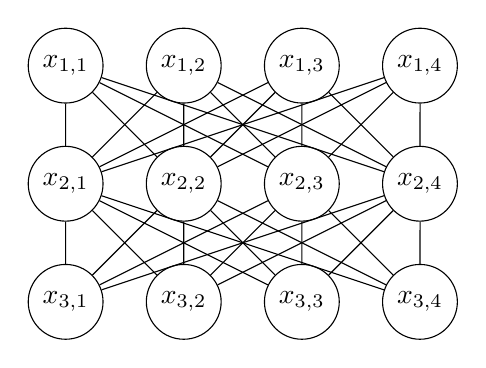
\begin{tikzpicture}[scale=1.5]
    % Define coordinates for nodes
    \foreach \x in {1,...,4} {
        \node[circle,draw] (x1\x) at (\x,2) {$x_{1,\x}$};
        \node[circle,draw] (x2\x) at (\x,1) {$x_{2,\x}$};
        \node[circle,draw] (x3\x) at (\x,0) {$x_{3,\x}$};
    }
    
    % Draw edges between nodes
    \foreach \x in {1,...,4} {
        \foreach \y in {1,...,4} {
            \draw (x1\x) -- (x2\y);
            \draw (x2\x) -- (x3\y);
        }
    }
\end{tikzpicture}

\end{document}